\section{Extended Toy and MNIST Experiments}
\label{app:extended_toy}

This appendix provides a deeper empirical analysis of the capacity mismatch and the REPA-\texorpdfstring{$\Sigma$}{Sigma} mechanism introduced in Section~\ref{sec:repa_sigma_experiments}. We focus on exactly \emph{when} gradient conflict occurs during the diffusion process, and whether the observed bias is a transient learning artifact or a permanent fixed-point alteration.

\paragraph{Robustness to Alignment Strength and Capacity Mismatch}
To understand how the capacity mismatch explicitly harms the denoiser, we simulated a diagonal linear denoiser trained on a synthetic data distribution. The distribution comprised semantic coordinates (a mixture of Gaussians) and detail coordinates (pure Gaussian noise). The teacher projection explicitly preserved the semantic coordinates while zeroing out the detail coordinates.

If the denoiser blindly follows the teacher, it should lose its ability to generate details. To test this, we swept the REPA alignment weight $\lambda$, tracking the final Total MSE of the model. 

As shown in Figure~\ref{fig:lambda_sweep_robustness}, standard REPA is highly brittle. As the alignment weight $\lambda$ increases, the model is forced to suppress details to match the teacher, causing the Total MSE to diverge catastrophically. By contrast, REPA-\texorpdfstring{$\Sigma$}{Sigma} dynamically projects out these conflicting, detail-suppressing gradients. As a result, it remains robust, maintaining near-optimal MSE even at high $\lambda$ values. This confirms that the gradient-surgery operator successfully isolates the teacher's useful semantic signal from its harmful detail-suppressing component.

\begin{figure}[htbp]
  \centering
  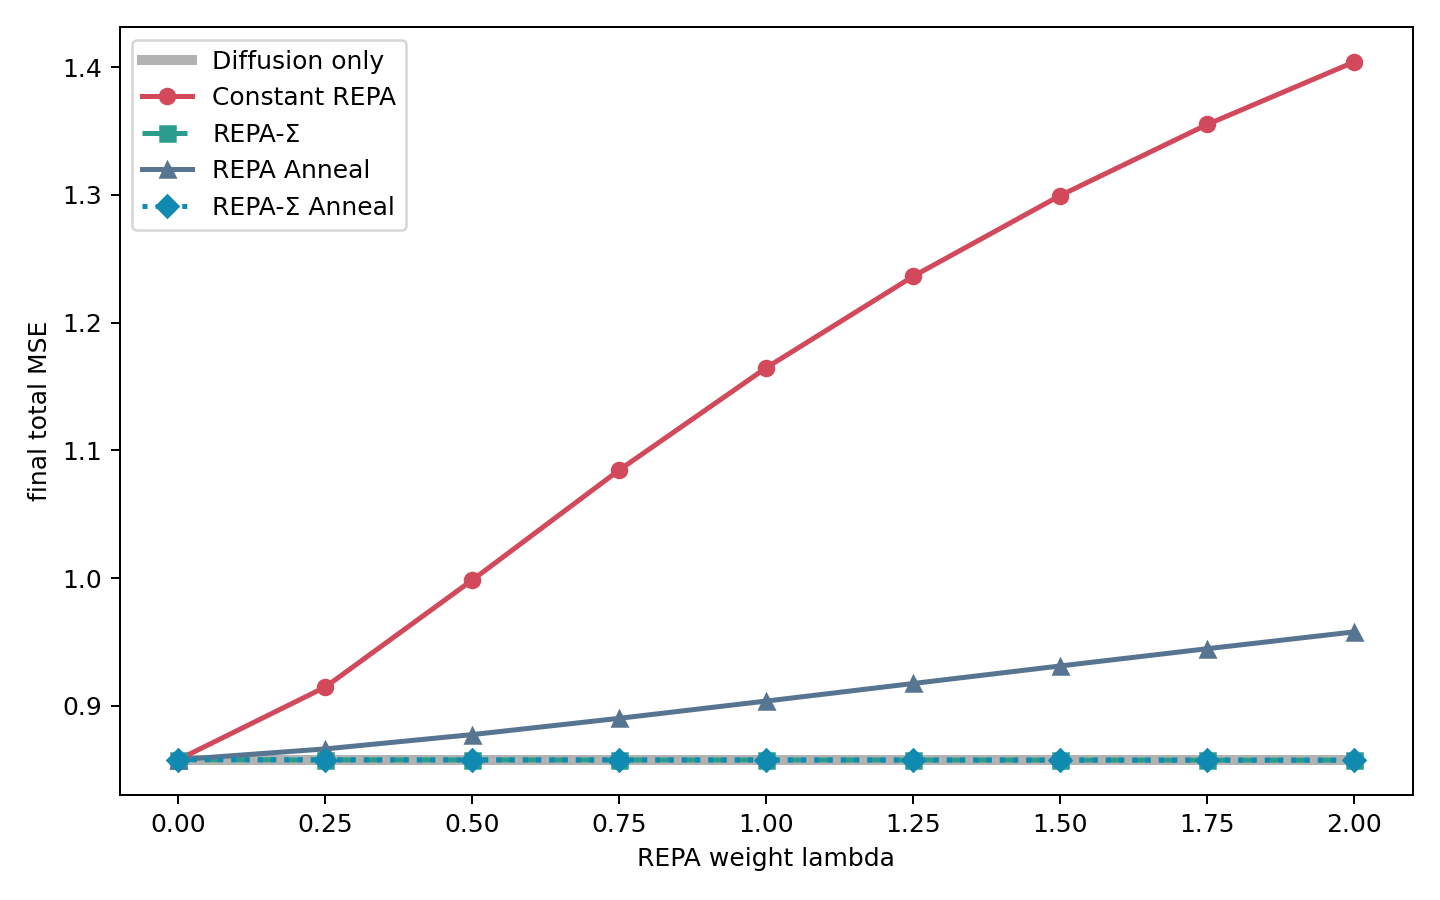
\includegraphics[width=0.8\linewidth]{images/fig_lambda_sweep_total_mse.png}
  \caption{Final Total MSE across a sweep of the alignment weight $\lambda$. Under standard REPA (red), forcing alignment with a teacher that discards details causes the error to explode. REPA-\texorpdfstring{$\Sigma$}{Sigma} (teal) dynamically removes the conflict, remaining robust even at high $\lambda$ values.}
  \label{fig:lambda_sweep_robustness}
\end{figure}

\paragraph{Long-Training Fixed-Point Proof}
A critical question when evaluating the blurry MNIST outputs (Figure~\ref{fig:mnist_samples}) is whether standard REPA simply learns high-frequency details \emph{slower}, or if the model's capacity to learn them is permanently destroyed.

We address this by training a non-linear Multi-Layer Perceptron (MLP) on MNIST for an extended 10,000-step regime (Figure~\ref{fig:mnist_long_training}). The results prove that standard REPA alters the fundamental fixed-point of the network: after 10,000 steps, its high-frequency (HF) MSE remains at 0.0091, permanently elevated above the pure diffusion baseline (0.0061). The effective HF gain similarly plateaus at 0.12, far below the baseline's 0.20. This confirms the bias is not a transient training artifact.

REPA-\texorpdfstring{$\Sigma$}{Sigma} reduces this permanent gap (HF MSE 0.0069, gain 0.15) but does not fully close it. It is only the combination of REPA-\texorpdfstring{$\Sigma$}{Sigma} with $\lambda$-annealing that eliminates the bias entirely: after 10,000 steps, REPA-\texorpdfstring{$\Sigma$}{Sigma} + anneal achieves HF MSE 0.0058 and gain 0.20, effectively matching the pure diffusion baseline (HF MSE 0.0061, gain 0.20). This definitively solves the capacity mismatch introduced by the teacher.

\begin{figure}[htbp]
  \centering
  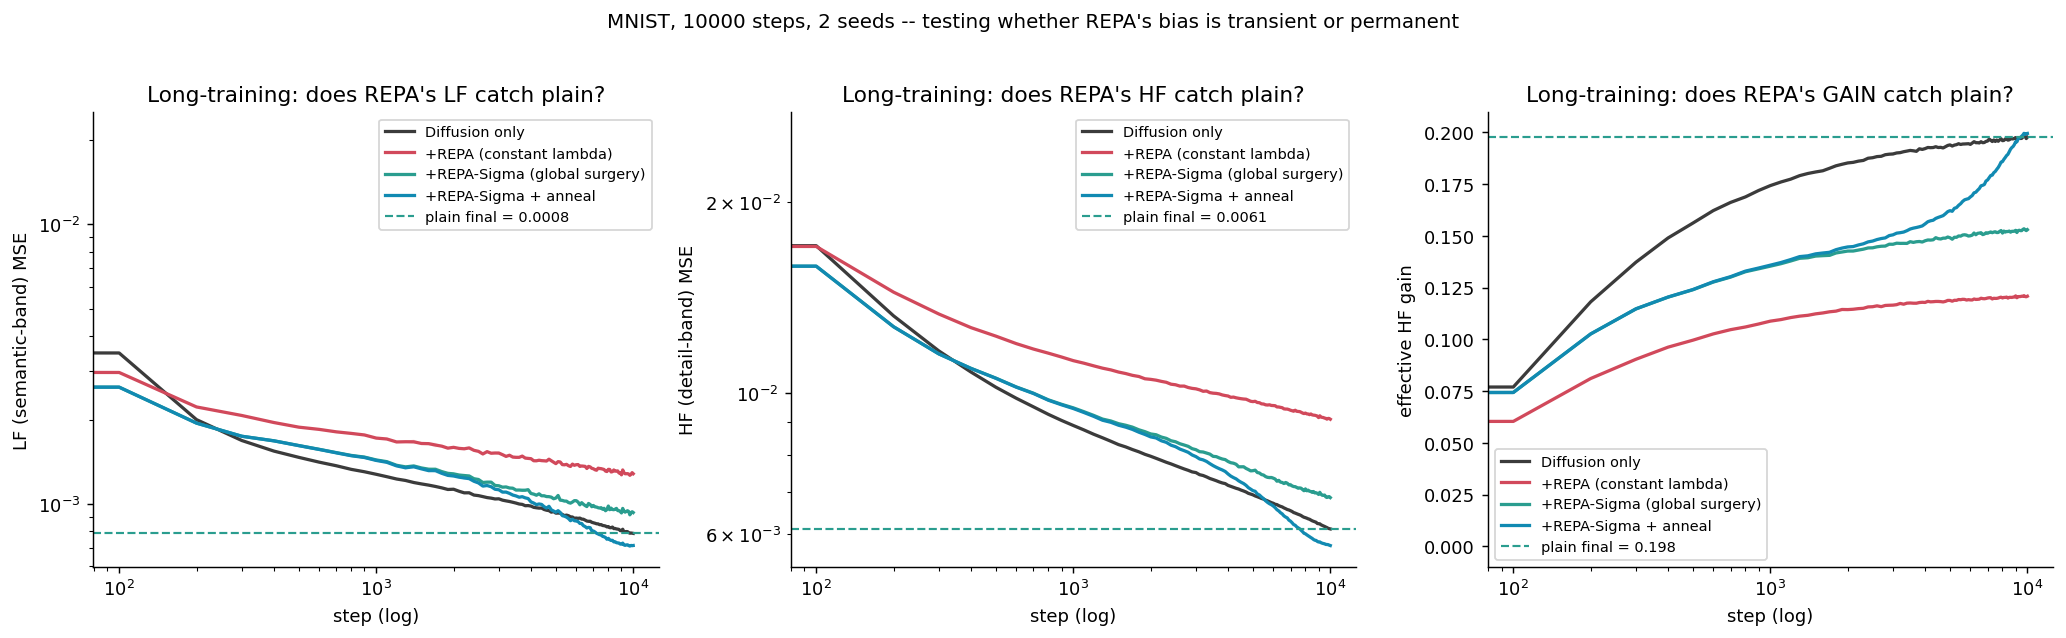
\includegraphics[width=\linewidth]{images/mnist_J_long.png}
  \caption{Extended 10,000-step training diagnostic on MNIST. Standard REPA exhibits a permanent gap in High-Frequency (HF) detail MSE, proving the bias is not a transient training artifact. REPA-\texorpdfstring{$\Sigma$}{Sigma} reduces the gap, but REPA-\texorpdfstring{$\Sigma$}{Sigma} combined with $\lambda$-annealing eliminates it entirely, converging to the unbiased fixed point.}
  \label{fig:mnist_long_training}
\end{figure}
